\documentclass[11pt,a4paper]{article}

\usepackage[utf8]{inputenc}
\usepackage[T1]{fontenc}
\usepackage{lmodern}
\usepackage[french]{babel}
\usepackage[margin=2.1cm]{geometry}
\usepackage{microtype}
\usepackage{amsmath,amssymb}
\usepackage{booktabs}
\usepackage{array}
\usepackage[table]{xcolor}
\usepackage{graphicx}
\usepackage{caption}
\usepackage[most]{tcolorbox}

\definecolor{navy}{HTML}{1F3864}
\definecolor{bluemid}{HTML}{2E5496}
\definecolor{lightblue}{HTML}{D6E0F0}

\captionsetup{font=small,labelfont={bf,color=navy},labelsep=period}
\graphicspath{{../figures/}}

\newtcolorbox{cle}[1][]{colback=lightblue!40,colframe=navy,boxrule=0.6pt,
  arc=2pt,left=8pt,right=8pt,top=6pt,bottom=6pt,#1}

\title{\vspace{-1.2cm}\color{navy}\bfseries La loi de comptage négative binomiale\\[2pt]
  \large Simulée, réconciliée, et son effet sur le capital}
\author{Kélian Kaddouri}
\date{27 juillet 2026}

\begin{document}
\maketitle
\vspace{-0.9cm}

\begin{cle}
\textbf{Le point à clarifier.} Le modèle porte \textbf{trois} représentations de la
surdispersion de la fréquence, à trois échelles, jamais confrontées~: la forme de mélange
Gamma $r=0{,}63$ au niveau firme (08b), la charge systémique $a=0{,}60$ de
\texttt{frequence\_model}, et le facteur négatif binomial $\varphi=9{,}20$ de la
configuration (moteur euro). Cette note montre par simulation que $a$ et $\varphi$ sont
\emph{la même} surdispersion vue à travers deux lois de mélange, mesure ce que le choix de
loi de comptage change au SCR, et cale $\varphi$ sur la vraie série.
\end{cle}

\medskip
\noindent\textbf{1. Réconciliation $a \leftrightarrow \varphi$.} Un Poisson mélangé a pour
indice de dispersion $\mathrm{Var}/\mathbb{E}$~: $1+\lambda/r=\varphi$ pour un mélange Gamma
(c'est la négative binomiale), $1+\lambda(e^{a^2}-1)$ pour un mélange lognormal. Les deux
décrivent \emph{la même} surdispersion si $e^{a^2}=1+(\varphi-1)/\lambda$, soit
$a=\sqrt{\ln(1+(\varphi-1)/\lambda)}$. À l'échelle du moteur euro ($\lambda\simeq 21{,}6$/an,
OpRisk), $\varphi=9{,}20$ correspond à $a=0{,}57$, très proche du $a=0{,}60$ posé~; et
$a=0{,}60$ implique $\varphi=10{,}3$. Les deux calages agrégés coïncident à $5\,\%$ près. Le
$r=0{,}63$ firme, lui, vit à l'échelle firme-année (dispersion $\simeq 1{,}16$) et ne se
compare pas directement.

\medskip
\begin{center}
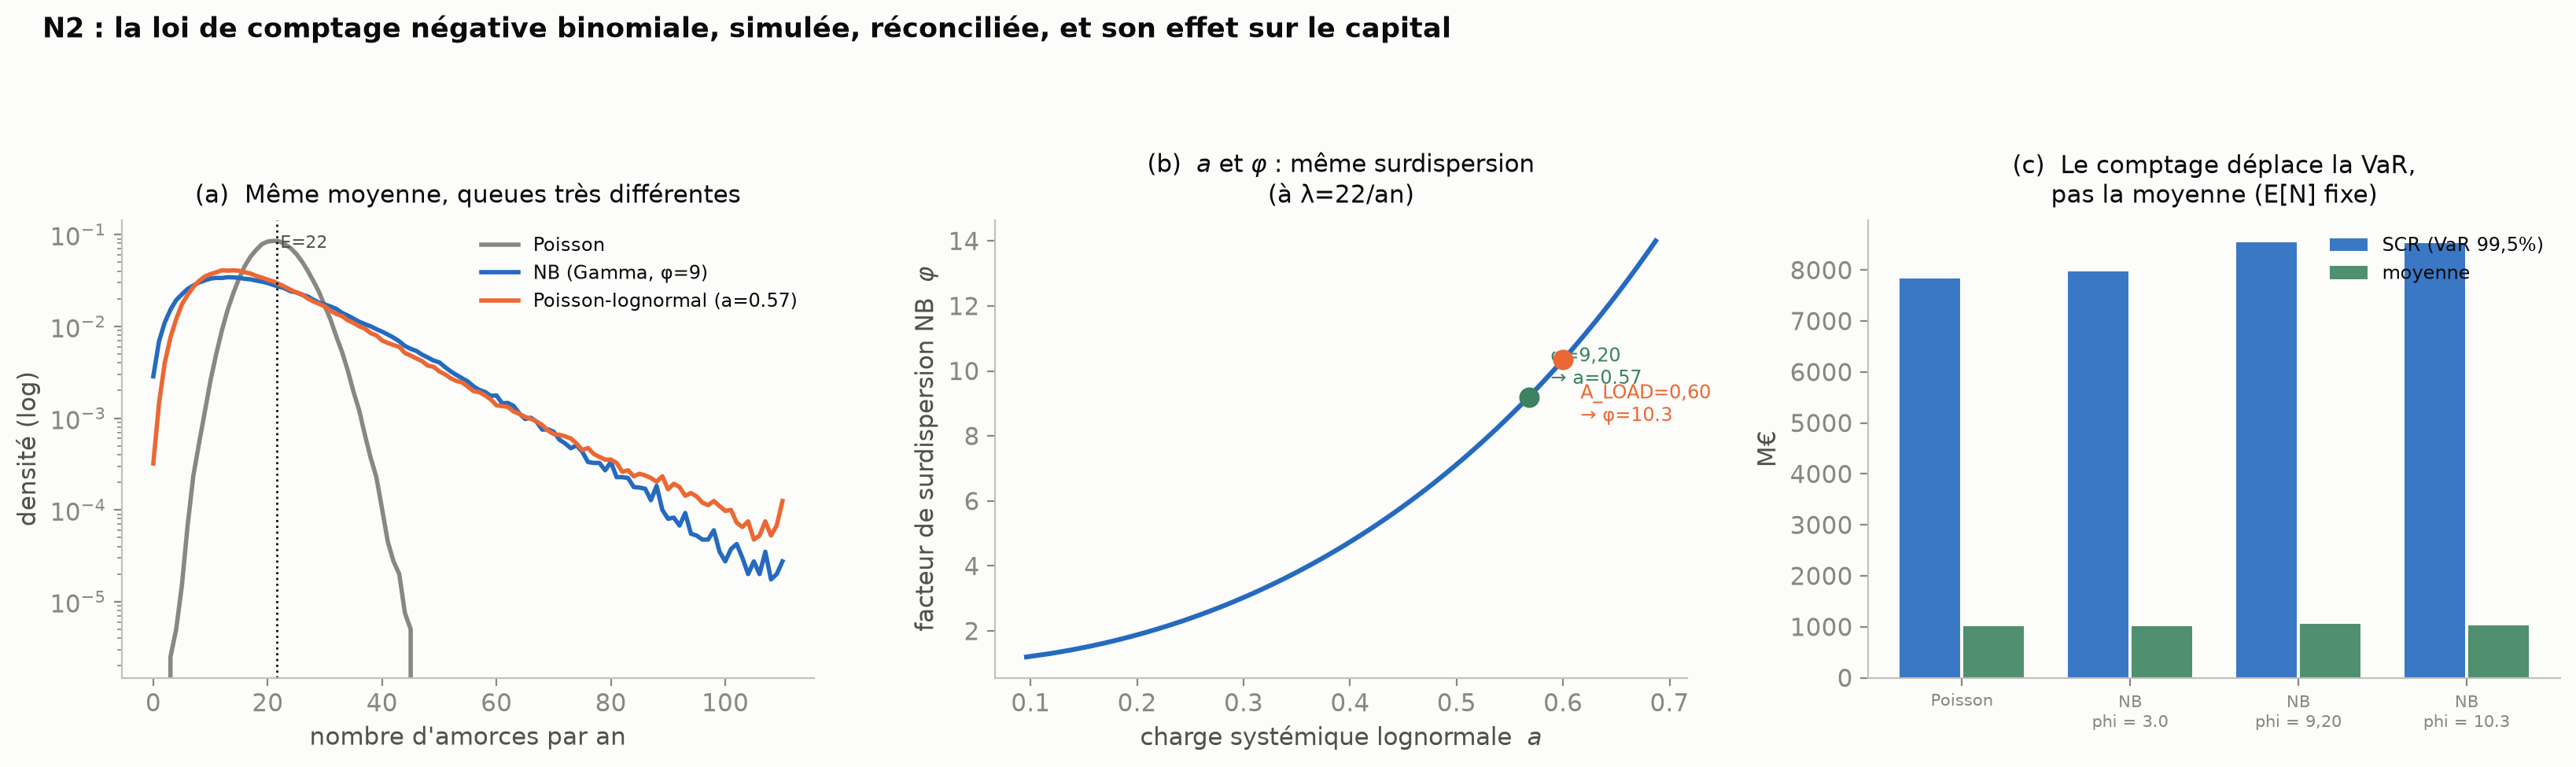
\includegraphics[width=\linewidth]{N2_simulation_nb.png}
\captionof{figure}{\textbf{(a)} à moyenne égale ($\lambda\simeq 22$), les queues diffèrent
fortement selon la loi de comptage. \textbf{(b)} la charge lognormale $a$ et le facteur NB
$\varphi$ tracent la même surdispersion, et les deux valeurs posées ($a=0{,}60$,
$\varphi=9{,}20$) quasi coïncident. \textbf{(c)} le comptage déplace la VaR mais pas la
moyenne (l'espérance $\mathbb{E}[N]=\lambda$ est fixe pour les trois lois).}
\end{center}

\begin{cle}
\textbf{Deux résultats à retenir.}
\begin{enumerate}\itemsep2pt
\item \textbf{Même variance, queue différente.} À indice de dispersion égal ($9{,}2$), le
quantile $99{,}5\,\%$ du nombre annuel vaut $74$ pour la négative binomiale (mélange Gamma)
contre $82$ pour le Poisson-lognormal, soit $+11\,\%$. Appairer la variance n'appaire pas la
queue~: la loi de mélange n'est pas neutre.
\item \textbf{Le comptage déplace la VaR, pas la moyenne.} La moyenne de perte est invariante
par construction. La surdispersion remonte la VaR de $+9\,\%$ (Poisson vers NB posée)~: effet
modéré, car au $99{,}5\,\%$ la queue reste portée par la perte unique dominante (sévérité
$\xi\simeq 0{,}60$), cohérent avec le script~29.
\end{enumerate}
\end{cle}

\begin{cle}[colback=orange!8,colframe=orange!70!black]
\textbf{Honnêteté sur le statut de $\varphi$.} En calant la charge sur la vraie série
cyber\,$\times$\,finance 2005-2022 \emph{détrendée} (le $\mathrm{Var}/\mathbb{E}$ brut confond
la croissance avec le choc commun, discipline du script~08b), on obtient $a\simeq 0{,}30$ et
$\varphi\simeq 3{,}0$, bien en deçà du $9{,}20$ posé. Le $\varphi$ de la configuration est
donc un \textbf{choix de prudence sur la queue de fréquence, pas une calibration}, et doit
être assumé comme tel. La négative binomiale (mélange Gamma) reste le bon objet agrégé~: forme
close, un seul paramètre, quantiles exacts.
\end{cle}

\smallskip
\noindent\footnotesize\textcolor{navy}{\textbf{Source.}} Script
\texttt{2\_donnees/41\_simulation\_nb\_comptage.py}, figure \texttt{N2\_simulation\_nb.png}.
Prolonge 08b (calibration firme) et 08d (Poisson composé).

\end{document}
